
\documentclass{beamer} 


\mode<presentation>
{
  \usetheme[hideothersubsections]{Berkeley}
  % or ...

  \setbeamercovered{transparent}
  % or whatever (possibly just delete it)
}

\usepackage{tikz}
\usetikzlibrary{decorations.pathreplacing,angles,quotes}
\usetikzlibrary{shapes, shadows, arrows, positioning,fit}\usepackage{graphicx}
\usepackage[english]{babel}
% or whatever

\usepackage[utf8]{inputenc}
% or whatever

\usepackage{times}
\usepackage[T1]{fontenc}
% Or whatever. Note that the encoding and the font should match. If T1
% does not look nice, try deleting the line with the fontenc.
\addtobeamertemplate{navigation symbols}{}{%
    \usebeamerfont{footline}%
    \usebeamercolor[fg]{footline}%
    \hspace{1em}%
    \insertframenumber/\inserttotalframenumber
}

\def\gray{\color{lightgray}}
\def\red{\color{red}}
\def\white{\color{white}}
\def\brown{\color{brown}}
\def\black{\color{black}}
\def\blue{\color{blue}}


\title[Open Policy Analysis ] % (optional, use only with long paper titles)
{Why We Need Open Policy Analysis}

\subtitle
{}

\author[] % (optional, use only with lots of authors)
{Fernando~Hoces de la Guardia\inst{1}\\
Sean~Grant\inst{2}\\
Edward Miguel\inst{1}}
% - Give the names in the same order as the appear in the paper.
% - Use the \inst{?} command only if the authors have different
%   affiliation.

\institute[Universities of Somewhere and Elsewhere] % (optional, but mostly needed)
{
  \inst{1}%
  UC Berkeley:\\
  Berkeley Initiative for Transparency in the Social Sciences\\
  \inst{2}%
  RAND\\
}
% - Use the \inst command only if there are several affiliations.
% - Keep it simple, no one is interested in your street address.

\date[] % (optional, should be abbreviation of conference name)
{Congressional Budget Office, March 2018\\
{\small Slides at} \url{http://www.github.com/fhoces/CBO2018}}
% - Either use conference name or its abbreviation.
% - Not really informative to the audience, more for people (including
%   yourself) who are reading the slides online

\subject{Research Transparency}
% This is only inserted into the PDF information catalog. Can be left
% out. 

\pgfdeclareimage[height=2cm]{university-logo}{../Images/BITSSlogo.png}
\logo{\pgfuseimage{university-logo}}

% If you have a file called "university-logo-filename.xxx", where xxx
% is a graphic format that can be processed by latex or pdflatex,
% resp., then you can add a logo as follows:

% \pgfdeclareimage[height=0.5cm]{university-logo}{university-logo-filename}
% \logo{\pgfuseimage{university-logo}}



% Delete this, if you do not want the table of contents to pop up at
% the beginning of each subsection:
%\AtBeginSubsection[]
%{
%  \begin{frame}<beamer>{Outline}
%    \tableofcontents[currentsection,currentsubsection]
%  \end{frame}
%}


% If you wish to uncover everything in a step-wise fashion, uncomment
% the following command: 

\beamerdefaultoverlayspecification{<.->}


\begin{document}

\begin{frame}
  \titlepage
\end{frame}




% Structuring a talk is a difficult task and the following structure
% may not be suitable. Here are some rules that apply for this
% solution: 

% - Exactly two or three sections (other than the summary).
% - At *most* three subsections per section.
% - Talk about 30s to 2min per frame. So there should be between about
%   15 and 30 frames, all told.

% - A conference audience is likely to know very little of what you
%   are going to talk about. So *simplify*!
% - In a 20min talk, getting the main ideas across is hard
%   enough. Leave out details, even if it means being less precise than
%   you think necessary.
% - If you omit details that are vital to the proof/implementation,
%   just say so once. Everybody will be happy with that.
%%%%%%%%%%%%%%%%%%%%%%%%%%%%%%%%%%%%%%%%%%%%%%%%%%%%%%%%%%%%%%%%%%%%%%%
%%%%%%%%%%%%%%%%%%%%%%%%%%%%%%%%%%%%%%%%%%%%%%%%%%%%%%%%%%%%%%%%%%%%%
\begin{frame}{Outline}
  \tableofcontents
  % You might wish to add the option [pausesections]
\end{frame}
 
 
\section[Evidence Based]{Policy Analysis And The Evidence-Based Policy Movement}

\begin{frame}{Policy Analysis And The Evidence-Based Policy Movement}
Evidence-Based Movement is Growing. 
\begin{itemize}
\item Haskins, (2017).
%\begin{itemize}
\item credible causal evidence (Angrist \& Pischke, 2010)
\item transparency and reproducibility of research (Miguel et al. 2014).
%\end{itemize} 
\item Commission on Evidence-Based Policymaking (CEBP)
\end{itemize}
\pause
Policy Analysis is fundamental link. 
\begin{itemize}
\item As many definitions as textbooks (Dunn, 2015; Weimer \& Vining, 2017; Williams, 1971)
\item Common denominator: client-oriented empirical analysis meant to inform a specific policy debate
\item Aspires at scientific rigor. (Wildavsky 1979),
\end{itemize}
\end{frame} 


\begin{frame}{An Ideal Evidence-Based Policy Link}



\tikzstyle{agent} = [diamond, draw, node distance= 7em, minimum height=5em, minimum width=5em]
\tikzstyle{line} = [draw, -stealth]

\tikzstyle{line_enph} = [draw, red, ultra thick]
\tikzstyle{inp} = [draw, circle, text centered, minimum height=2em, text width=2em, node distance= 10em]
\tikzstyle{outp} = [draw, circle, text centered, minimum height=2em, text width=2em, node distance= 10em]
\tikzstyle{block1} = [draw, circle,  text width=5em, text centered, minimum height=7em, node distance= 5em]
\tikzstyle{block2} = [draw, circle,  text width=7em, text centered, minimum height=2em, node distance= 5em]
\tikzstyle{block3} = [draw, rounded rectangle,  text width=5em, text centered, minimum height=2em, node distance= 5em]


\begin{figure}[h!]\centering
\vspace{-2.0em}
\begin{tikzpicture}[thick,scale=0.55, every node/.style={scale=0.55}]

%% The oddly shaped truth
\node[regular polygon, regular polygon sides=3,
              draw, fill=white,
              inner sep=.1em,
              shape border rotate=70](tru){Truth};


%%%%%Researcher 1 and Inputs: depends on R_1%%%%%%%
\node [block1, right = 2em of tru](R_1){Research\linebreak $(R)$};
\node [block1,inner sep=0em, right = 2em of R_1](PA_1){Policy \linebreak Analysis: ($PA$) \linebreak  Gains  \& \linebreak losses};
\node [block1, above right = 0em and 8em of R_1](PM_1){Policy\linebreak Maker 1};
\node [block1, below right = 0em and 8em of R_1](PM_2){Policy\linebreak Maker 2};

\node [block3, right = 2em of PM_1](PC_1){Support};
\node [block3, right = 2em of PM_2](PC_2){Oppose};


%%%%% Draw edges col 2%%%%%%%%%%%%%%%%%
%Research  to PA
\draw [line](tru) -- (R_1);
\draw [line](R_1) -- (PA_1);
%PA to PM
\draw [line](PA_1) -- (PM_1);
\draw [line](PA_1) -- (PM_2);
%PM to PC
\draw [line](PM_1) -- (PC_1);
\draw [line](PM_2) -- (PC_2);

%%%%%%%%%%%%%%%%%%%%%%%%%%%%%%%%%%%%%%



\draw[decoration={brace}, decorate] (7,3.4) -- node[above=6pt](lab4){{\Large Observed by citizens} }(16,3.4);




\end{tikzpicture}
\vspace{-.8em}
\end{figure}
\end{frame}


\section[Crisis in Research]{Reproducibility Crisis In Empirical Research}

\begin{frame}{Reproducibility Crisis In Empirical Research}

\begin{itemize}
\item  Researchers believe in good science but don't practices it (Anderson, Martinson, \& De Vries 2007).  
%\pause
%\item ``Most published research is false'' Ioannidis (2005). 
\pause
\item The file drawer problem is big (Franco et al 2014).  
\pause
\item Evidence of extensive p-hacking across social science disciplines (Gerber et al 2008, Brodeur et al 2016).
\pause
\item  Replication rates are low (Collaboration et al, 2015 40-60\%, Camerer et al, 2016 60\%). Computational reproducibility is also low (Stodden et al 2016, Chang and Li 2015 45\%, Gertler et al 2018 14\%).
\end{itemize}

\end{frame} 


\section[Open Science]{The Open Science Movement}

\begin{frame}{The Open Science Movement}

\begin{itemize}
\item Definition of principles of Open Science/Research Transparency (Miguel et al 2014)
\item Development of guidelines to operationalize principles of Open Science (Nosek et al 2015)
\item Journals and funders are responding to this: Registries (AEA), Journals (Science + 5k), Funders (CITE FUNDERS)
\end{itemize}

\end{frame} 

\section[Crisis in PA]{Credibility Crisis Of Policy Analysis}

\begin{frame}{Credibility Crisis Of Policy Analysis}
\begin{itemize}
\item Manski 
\item Report wars 
\item  RDOF(Simmons, Nelson, and Simonsohn 2011,Wicherts et al., 2016).
\end{itemize}
\end{frame} 

\begin{frame}[shrink=30]{How This Affects The Evidence Based Policy Link?}

\tikzstyle{agent} = [diamond, draw, node distance= 7em, minimum height=5em, minimum width=5em]
\tikzstyle{line} = [draw, -stealth]

\tikzstyle{line_d} = [draw, dashed, -stealth]
\tikzstyle{inp} = [draw, circle, text centered, minimum height=2em, text width=2em, node distance= 10em]
\tikzstyle{outp} = [draw, circle, text centered, minimum height=2em, text width=2em, node distance= 10em]
\tikzstyle{block1} = [draw, circle,  text width=3em, text centered, minimum height=2em, node distance= 5em]
\tikzstyle{block2} = [draw, circle,  text width=4em, text centered, minimum height=2em, node distance= 5em]
\tikzstyle{block3} = [draw, rounded rectangle,  text width=5em, text centered, minimum height=2em, node distance= 5em]

\begin{figure}[h!]
\centering
\hspace*{0.2\linewidth}
\begin{tikzpicture}[thick,scale=0.2, every node/.style={scale=0.8}]

%% The oddly shaped truth
\node[regular polygon, regular polygon sides=3,
              draw, fill=white,
              inner sep=.1em,
              shape border rotate=70](tru){Truth};


%%%%%Researcher 1 and Inputs: depends on R_1%%%%%%%
\node [block1, right = 5em of tru](R_2){$R_2$};
\node [block1, above = 8em of R_2](R_1){$R_1$} node [left = -0.1em of R_1, text width = 5em]{Large Treatment Effect};
\node [block1, below = 8em of R_2](R_3){$R_3$} node [left = -0.1em of R_3, text width = 5em]{Small Treatment Effect};

\draw[decoration={brace,mirror}, decorate] (13,-33) -- node[below=6pt, text width = 4.8em](lab1){Researchers Degrees of 
Freedom}(18,-33);

\draw[decoration={brace,mirror}, decorate] (29,-33) -- node[below=6pt, text width = 5em](lab2){Policy Analyst Degrees of 
Freedom}(34,-33);

\draw[decoration={brace}, decorate] (31,33) -- node[below=2pt]{Observed by citizens}(70,33);

%\node [agent](Researcher_1){$R_1$} node [left = 0.6em of Researcher_1, text width = 8em]{Large Treatment Effect};

\node [block1, right = 5em of R_1](PA_12){$PA_{1,2}$};
\node [block1, above = .5em of PA_12](PA_11){$PA_{1,1}$} node [right = -0.1em of PA_11, text width = 5em]{Large gains only};
\node [block1, below = .5em of PA_12](PA_13){$PA_{1,3}$};

\node [block1, right = 5em of R_2](PA_22){$PA_{22,}$};
\node [block1, above = .5em of PA_22](PA_21){$PA_{2,1}$};
\node [block1, below = .5em of PA_22](PA_23){$PA_{2,3}$};

\node [block1, right = 5em of R_3](PA_32){$PA_{3,2}$};
\node [block1, above = .5em of PA_32](PA_31){$PA_{3,1}$};
\node [block1, below = .5em of PA_32](PA_33){$PA_{3,3}$} node [right = -0.1em of PA_33, text width = 5em]{Large losses only};


\node [block2, above right = 3em and 15em of R_2](PM_1){Policy\linebreak Maker 1};
\node [block2, below right = 3em and 15em of R_2](PM_2){Policy\linebreak Maker 2};

\node [block3, right = 3em of PM_1](PC_1){Support};
\node [block3, right = 3em of PM_2](PC_2){Oppose};


%%%%% Draw edges col 2%%%%%%%%%%%%%%%%%
%Truth to research
\draw [line](tru) -- (R_1);
\draw [line_d](tru) -- (R_2);
\draw [line_d](tru) -- (R_3);


%Research  to PA
\draw [line_d](R_1) -- (PA_13);
\draw [line_d](R_1) -- (PA_11);
\draw [line](R_1) -- (PA_12);

\draw [line_d](R_2) -- (PA_23);
\draw [line_d](R_2) -- (PA_21);
\draw [line_d](R_2) -- (PA_22);

\draw [line_d](R_3) -- (PA_33);
\draw [line_d](R_3) -- (PA_31);
\draw [line_d](R_3) -- (PA_32);



%PA to PM
\draw [line](PA_11) -- (PM_1);
\draw [line](PA_33) -- (PM_2);
%PM to PC
\draw [line](PM_1) -- (PC_1);
\draw [line](PM_2) -- (PC_2);

%%%%%%%%%%%%%%%%%%%%%%%%%%%%%%%%%%%%%%




\end{tikzpicture}
\end{figure}
%\end{comment}
\end{frame}


\begin{frame}{Relevance 1: Cherry Picking Evidence}
\pause
\begin{exampleblock}{}
  {\large ``When I was director of the CBO, I was very frustrated when we would write a policy report [saying] a certain policy would have these two advantages and these two disadvantages, and the advocates would quote only the part about the advantages, and the opponents would quote only the part about the disadvantages. That encourages the view that there are simple answers. There aren't generally simple answers. There are trade-offs.''
%I would strayed from Josh Angrist.. what is the right word... [DC says] straight jacket (in a friendly tone). That is a %good one. Although if I were to have a hierarchy of what is the strongest, I would probably start wearing Josh's straight %jacket
}
  \vskip3mm
  \raggedleft{\small--- Douglas Elmendorf (Director of CBO, 2009-2015)} \footnotesize{ \linebreak  Harvard Magazine, 2016} 
  	  
\end{exampleblock}
\end{frame} 

%6mins
\begin{frame}[shrink=25, label = pa_comp]{Relevance 2: Challenging to Automate and Improve Systematically Recurring Reports}

\tikzstyle{estimate} = [diamond, draw, node distance= 7em,text width = 5em, minimum height=5em, minimum width=5em, align = center]
\tikzstyle{line} = [draw, -stealth]
\tikzstyle{line_enph} = [draw, red, ultra thick]
\tikzstyle{inp} = [draw, rectangle, text centered, minimum height=3em, text width=2em, node distance= 2em]
\tikzstyle{source} = [draw, rectangle, text centered, minimum height=8em, text width=5em, node distance= 10em]
\tikzstyle{model} = [draw, rectangle, text centered, minimum height=8em, text width=15em, node distance= 10em]
%\tikzstyle{outp} = [draw, ellipse, text centered, minimum height=2mm, text width=2em, node distance= 10em]
%\tikzstyle{block} = [draw, rectangle,  text width=8em, text centered, minimum height=55mm, node distance= 5em]


%\begin{adjustbox}{max totalsize={1\textwidth}{.8\textheight},center}

\begin{figure}[h!]\centering 
\hspace*{-2.5em}
\begin{tikzpicture}[thick,scale=0.6, every node/.style={scale=0.6}]
\setbeamercovered{invisible}

%%%%%Nodes: Sources%%%%%%%
\node [source](D_1){$Data$};
\node [source, below = 1em of D_1](Lit){$Research$};
\node [source, below = 1em of Lit](OR){\textit{Guess work}};


\draw[decoration={brace,mirror}, decorate] (-1.2,-10) -- node[below=6pt] {$Sources$}(1.1,-10);

\draw[decoration={brace,mirror}, decorate] (4.8,-11.3) -- node[below=6pt] {$Inputs$}(6.2,-11.3);


%node[below = 1em ](OR) -- node[below = 6em]{asd}(OR)


%\onslide<2-5>\node [source, color=red](Lit){$Research$};

%%%%%Nodes: Inputs%%%%%%%
\node [inp, above right = 1em and 6em of  D_1 ](I_1){$I_1$};
\node [inp, below = 1em of I_1](I_2){$I_2$};
\node [inp, below = 8em of I_2](I_j){$I_j$};
\node [inp, below right = 1em and 6em of OR ](I_last){$I_J$};




\path (I_2) -- node[auto=false, rotate=90, anchor=north, outer sep=-0.5em]{\ldots} (I_j);
\path (I_j) -- node[auto=false, rotate=90, anchor=north, outer sep=-0.5em]{\ldots} (I_last);

%%%%%Paths connecting Sources with Inputs%%%%%%%
\draw [line](D_1.east) -- (I_1.west);
\draw [line](D_1.east) -- (I_2.west);
\draw [line, opacity=1, anchor=center](Lit.east) -- (I_j.west);
\draw [line, opacity=1, anchor=center](OR.east) -- (I_last.west);


\draw [line, opacity=.3][xshift=1em](D_1.east) -- ([yshift=-8 em]I_1.west);
\draw [line, opacity=.3][xshift=1em](D_1.east) -- ([yshift=-10 em]I_1.west);

\draw [line, opacity=.3][xshift=1em](Lit.east) -- ([yshift=7 em]I_j.west);
\draw [line, opacity=.3][xshift=1em](Lit.east) -- ([yshift=-5 em]I_j.west);

\draw [line, opacity=.3][xshift=1em](OR.east) -- ([yshift=3 em]I_last.west);
\draw [line, opacity=.3][xshift=1em](OR.east) -- ([yshift=5 em]I_last.west);


%%%%%Node and paths for model%%%%%%%
\node [model, below right = 2em and 10em of D_1](model){$Model$};
\draw [line](I_1) -| (model);
\draw [line](I_2) -| (model);
\draw [line](I_j) |- (model);
\draw [line](I_last) -| (model);


%%%%%Node and paths for policy estimates%%%%%%%
\node [estimate, right = 5em of model](PE_2){$Policy$ $Estimate_2$};
\node [estimate, above = 5em of PE_2](PE_1){$Policy$ $Estimate_1$};
\node [estimate, below = 5em of PE_2](PE_3){$Policy$ $Estimate_3$};


\draw [line] (model.east) -- (PE_1.south west);
\draw [line] (model.east) -- (PE_2.west);
\draw [line] (model.east) -- (PE_3.north west);


\end{tikzpicture}
\end{figure}

\end{frame}

\begin{frame}{Relevance 3: Difficulty Understanding how Research Informs Policy Analysis}
\begin{itemize}
\item What happens when new research emerges?
\item Where a the largest unknowns in the policy analysis?
\item Where is the marginal piece of research most informative for this analysis?
\end{itemize}
\end{frame} 

\section[Open PA]{Proposed Principles for Open Policy Analysis}

\begin{frame}{Open Policy Analysis}
\begin{table}[ht]
\centering
\begin{tabular}[t]{|l|c|c|}
\hline
& Empirical  & Policy \\
& Research & Analysis \\

\hline
Problems & Reproducibility  &  Credibility \\
				 &  Crisis & Crisis \\
\hline
Solutions &  \textit{Open Science }&    {\white \textit{Open Policy Analysis } }\\
 & Principles, Guidelines,  &   {\white Principles, Guidelines,}\\
 & Applications &   {\white Applications}\\

\hline
\end{tabular}
\end{table}%
\end{frame}

\begin{frame}[noframenumbering]{Open Policy Analysis}
\begin{table}[ht]
\centering
\begin{tabular}[t]{|l|c|c|}
\hline
& Empirical  & Policy \\
& Research & Analysis \\

\hline
Problems & Reproducibility  &  Credibility \\
				 &  Crisis & Crisis \\
\hline
Solutions &  \textit{Open Science }&    \textit{Open Policy Analysis } \\
 & Principles, Guidelines,  &   Principles\\
 & Applications &   \\

\hline
\end{tabular}
\end{table}%
\end{frame}

\begin{frame}{Principles for Open Policy Analysis}
Proposed principles:
\begin{enumerate}
\item Computational Reproducibility
\item Analytic Transparency
\item Output Transparency 
\end{enumerate}
\end{frame} 

\begin{frame}{Principle 1}
\begin{columns}
\begin{column}{0.3\textwidth}
\textbf{Computational Reproducibility}
\begin{itemize}
\item Literate \\ Programming
\item Version control
\item File structure
\item Label sources
\end{itemize}
\end{column}
\begin{column}{0.7\textwidth}  %%<--- here
    \begin{center}
     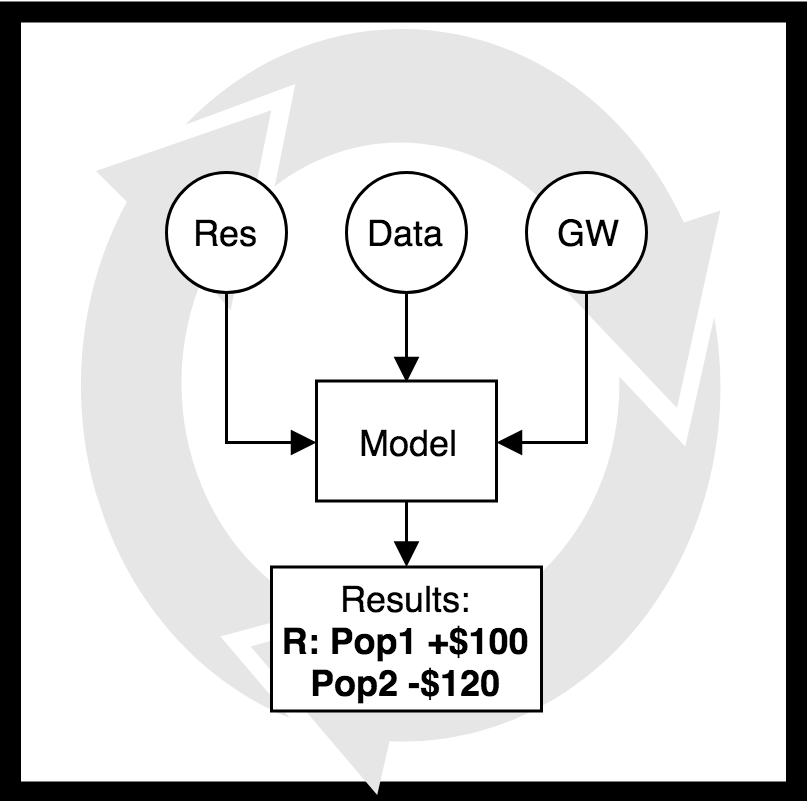
\includegraphics[width=1\textwidth]{../Images/repro.png}
     \end{center}
\end{column}
\end{columns}
\end{frame}

\begin{frame}{Principle 2}
\begin{columns}
\begin{column}{0.3\textwidth}
   \textbf{Analytic Transparency}
   \begin{itemize}
   \item Open code
   \item Open data
   \item  Report as Dynamic Document    
   \end{itemize}
\end{column}
\begin{column}{0.7\textwidth}  %%<--- here
    \begin{center}
     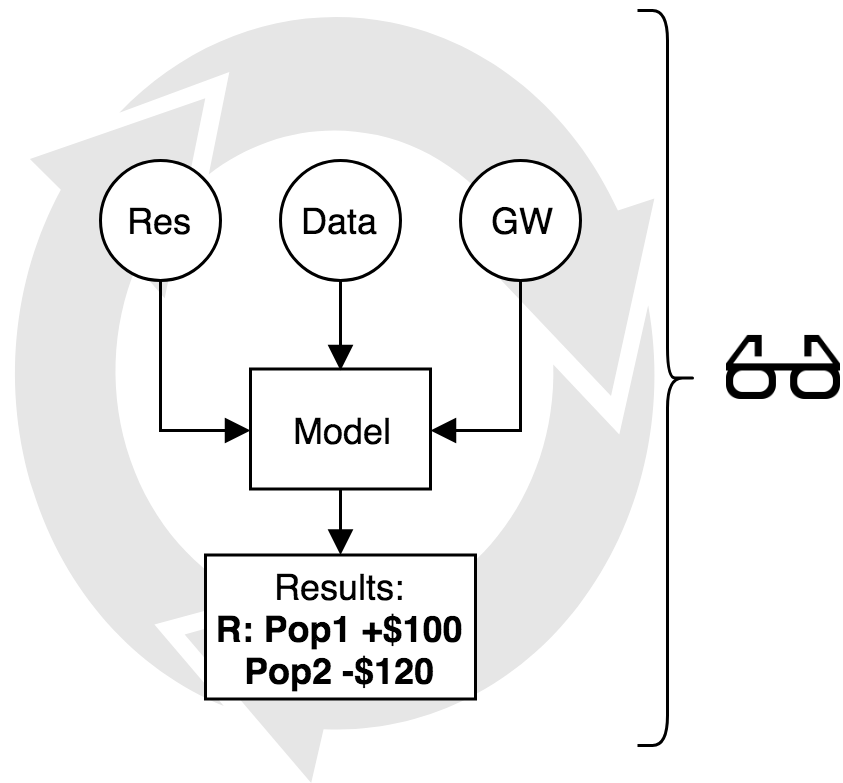
\includegraphics[width=1\textwidth]{../Images/a_transp.png}
     \end{center}
\end{column}
\end{columns}
\end{frame}

\begin{frame}{Principle 3}
\begin{columns}
\begin{column}{0.3\textwidth}
 \textbf{Output \\ Transparency}
   \begin{itemize}
   \item Pre-committed output display
   \item Assumptions-output link
   \end{itemize}
\end{column}
\begin{column}{0.7\textwidth}  %%<--- here
    \begin{center}
    \vspace{-2em}
     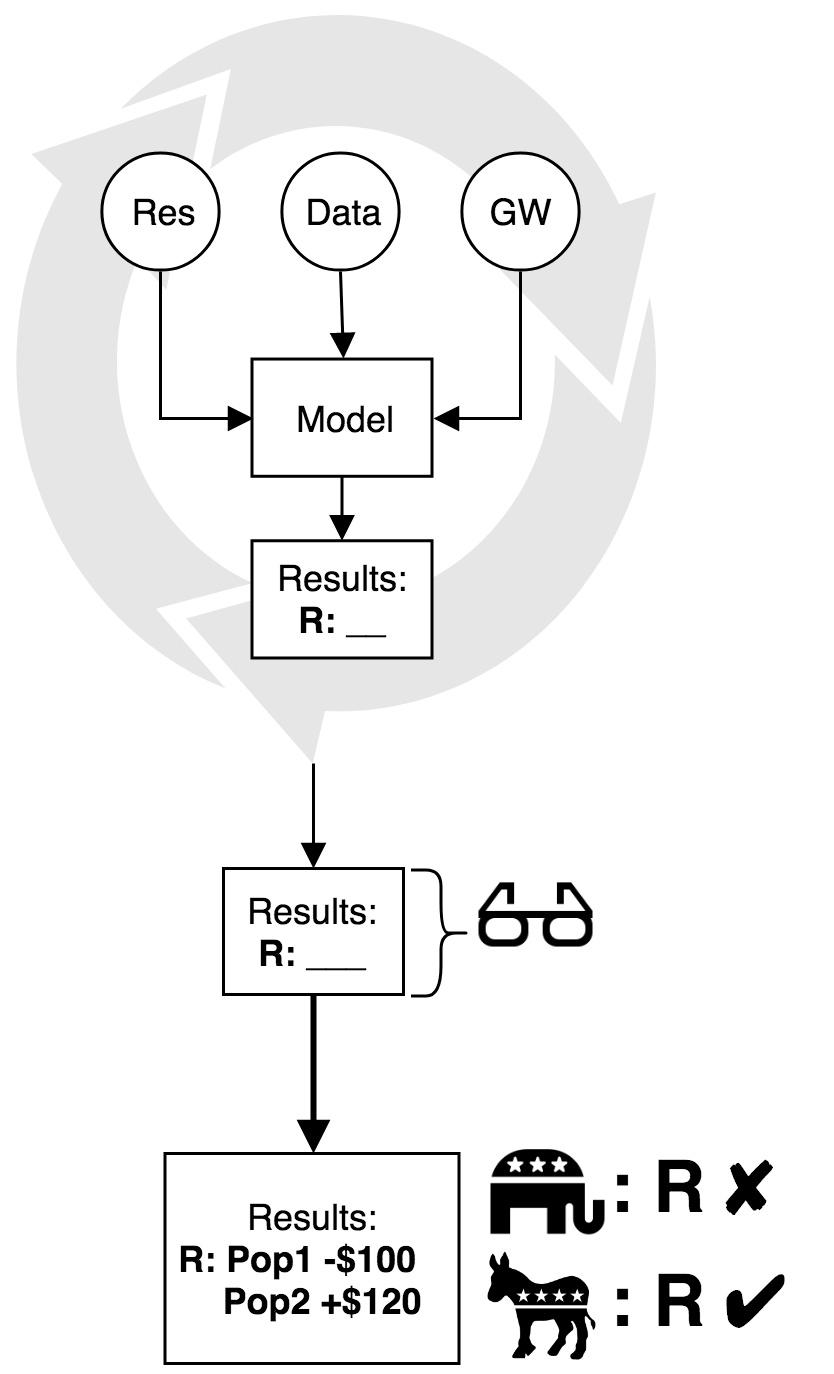
\includegraphics[width=.6\textwidth]{../Images/o_transp.png}
     \end{center}
\end{column}
\end{columns}
\end{frame}


\section{Challenges And Suggestions}

\begin{frame}{Challenges And Suggestions}
\textbf{Challenges:}
\begin{itemize}
\item Policymakers may not want analyses to be open.
\item Analysts may wish to keep policy analyses ``closed''. 
\item For policy analysis contracted out to third parties: Opening methods will prevent them form reselling extensions.
\item  Initially reproducibility represents an additional layer of work.
\item Limits to sharing sensitivity of information, requires resources for adequate de-identification if open data is expected
\end{itemize}
\end{frame} 

\begin{frame}{Challenges And Suggestions}
\textbf{Suggestions:}
\begin{enumerate}
\item \textbf{Policy Analysts: Just Post It}. \\
Things are moving in this direction. Play a leading role in a credibility revolution for policy analysis. Examples: from science.
\pause 
\item \textbf{Policy Analysis Organizations: Open by Default} \\
Boost in credibility, lower costs in the long run. First mover advantage. Examples: GiveWell, and AEI. 
\pause 
\item \textbf{Government Agencies and Funders: Support Open Policy Analysis}
Examples: Require contracted policy analysis to be fully open. Support training and adoption of new tools (VC and DD). Inject resources for the transition. Examples: from science.
\end{enumerate}
\end{frame} 


\section[Conclusion]{Conclusion And Next Steps}

\begin{frame}{Summing Up: Where We Are}
   \begin{tikzpicture}[remember picture,overlay]
       \node[at=(current page.center), xshift = 3.3em, yshift = -1.4em] {
         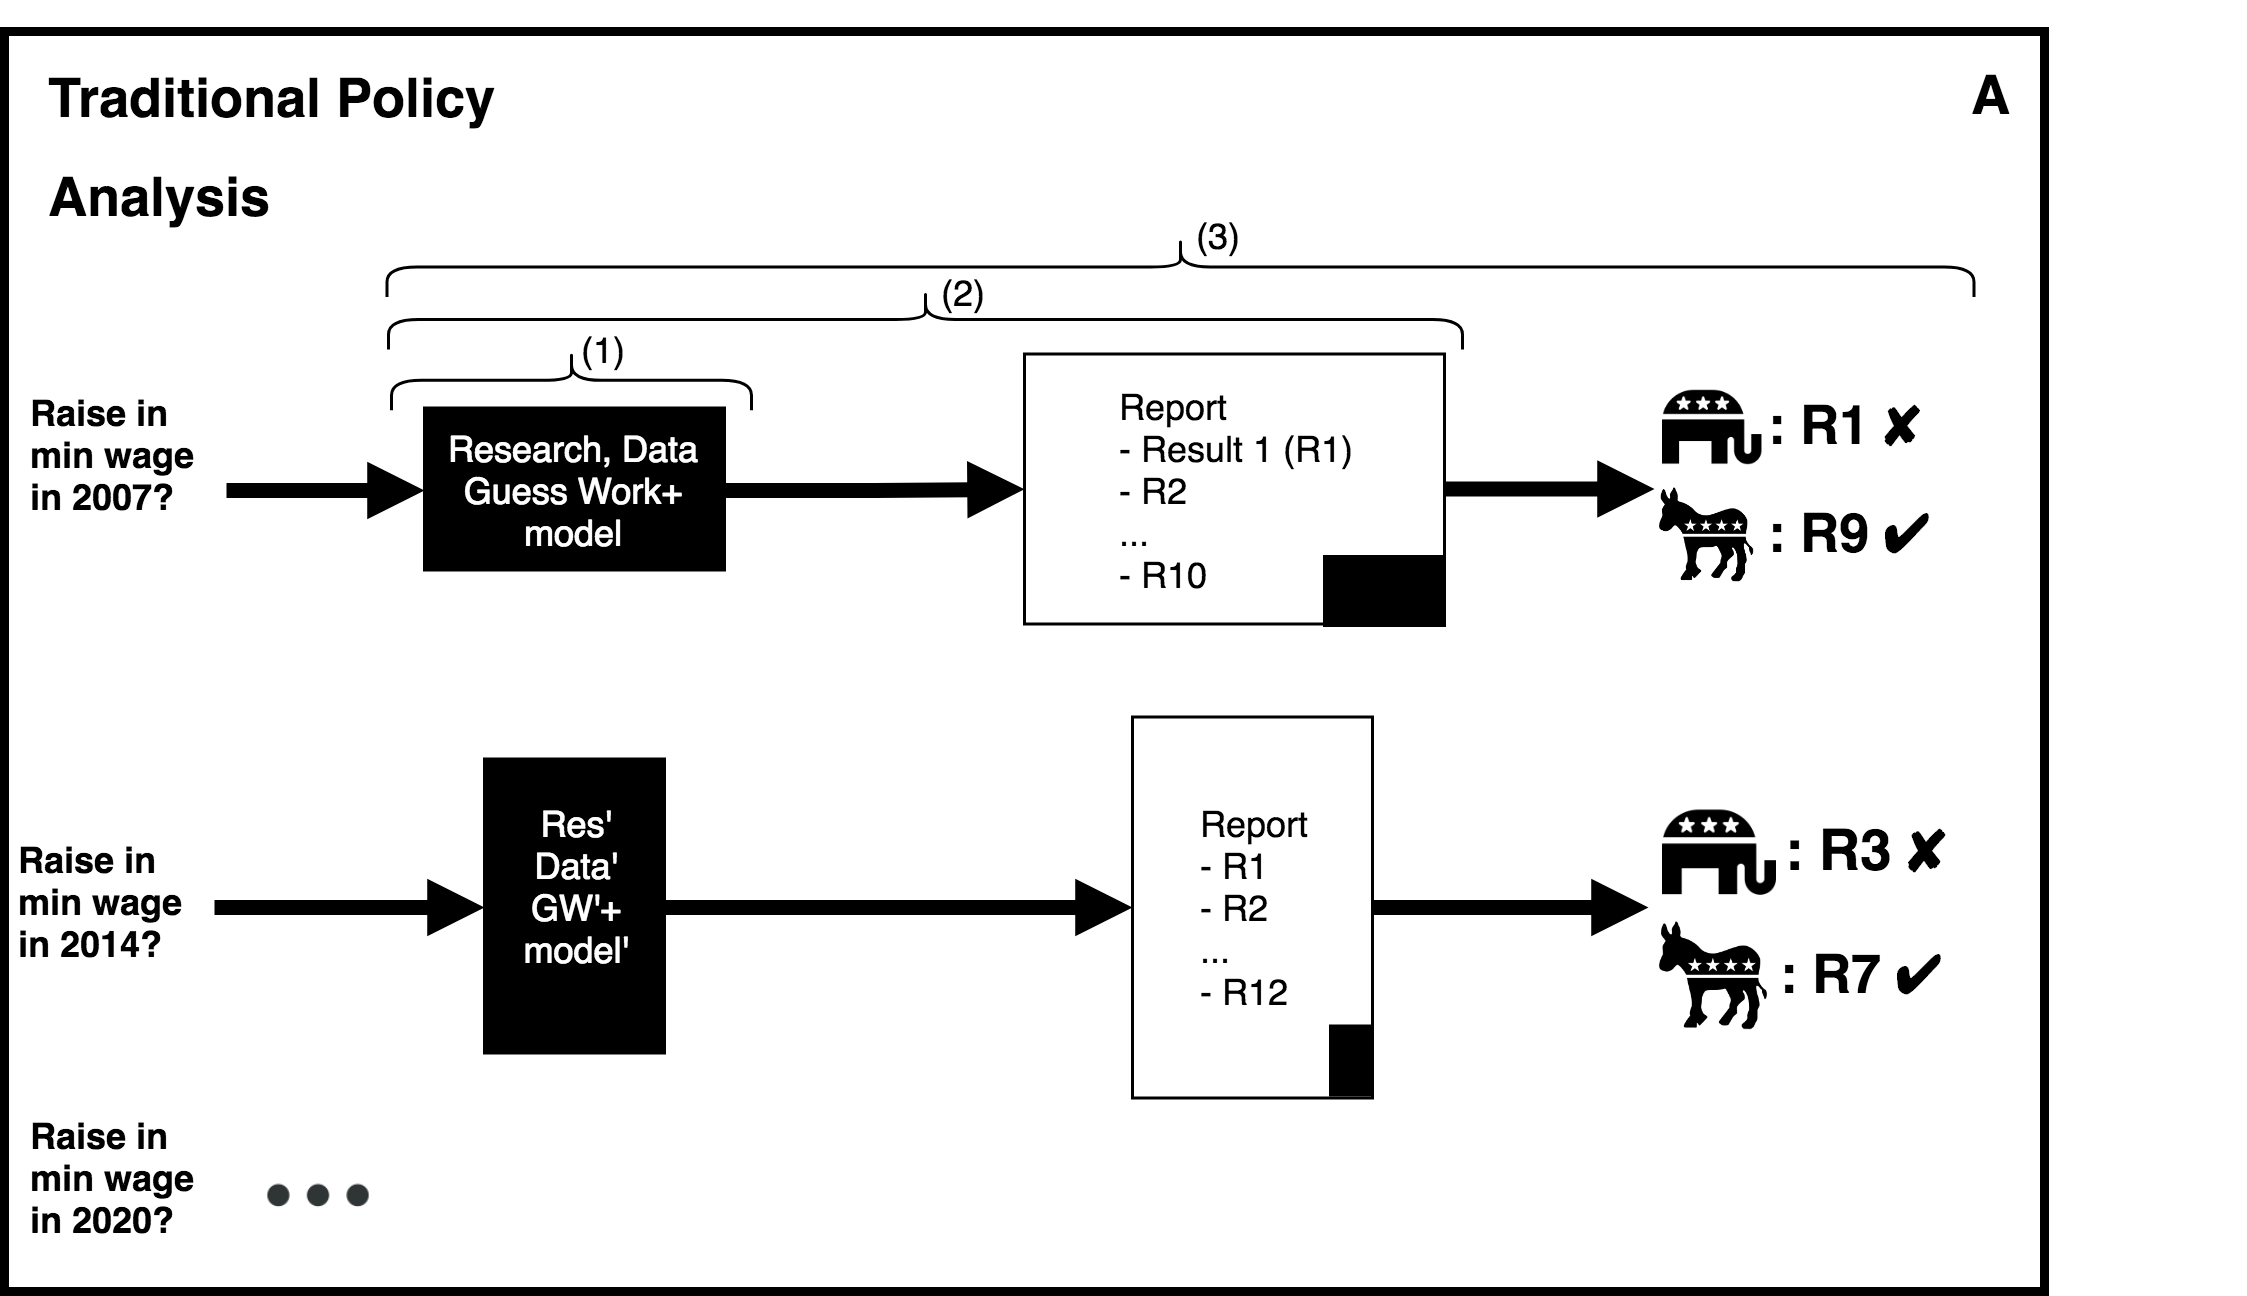
\includegraphics[width=.94\paperwidth]{../Images/traditional_pa.PNG}
       };
   \end{tikzpicture}
\end{frame}

\begin{frame}{Summing Up: Where Should We Go}
   \begin{tikzpicture}[remember picture,overlay]
       \node[at=(current page.center), xshift = 2em, yshift = -1.4em] {
         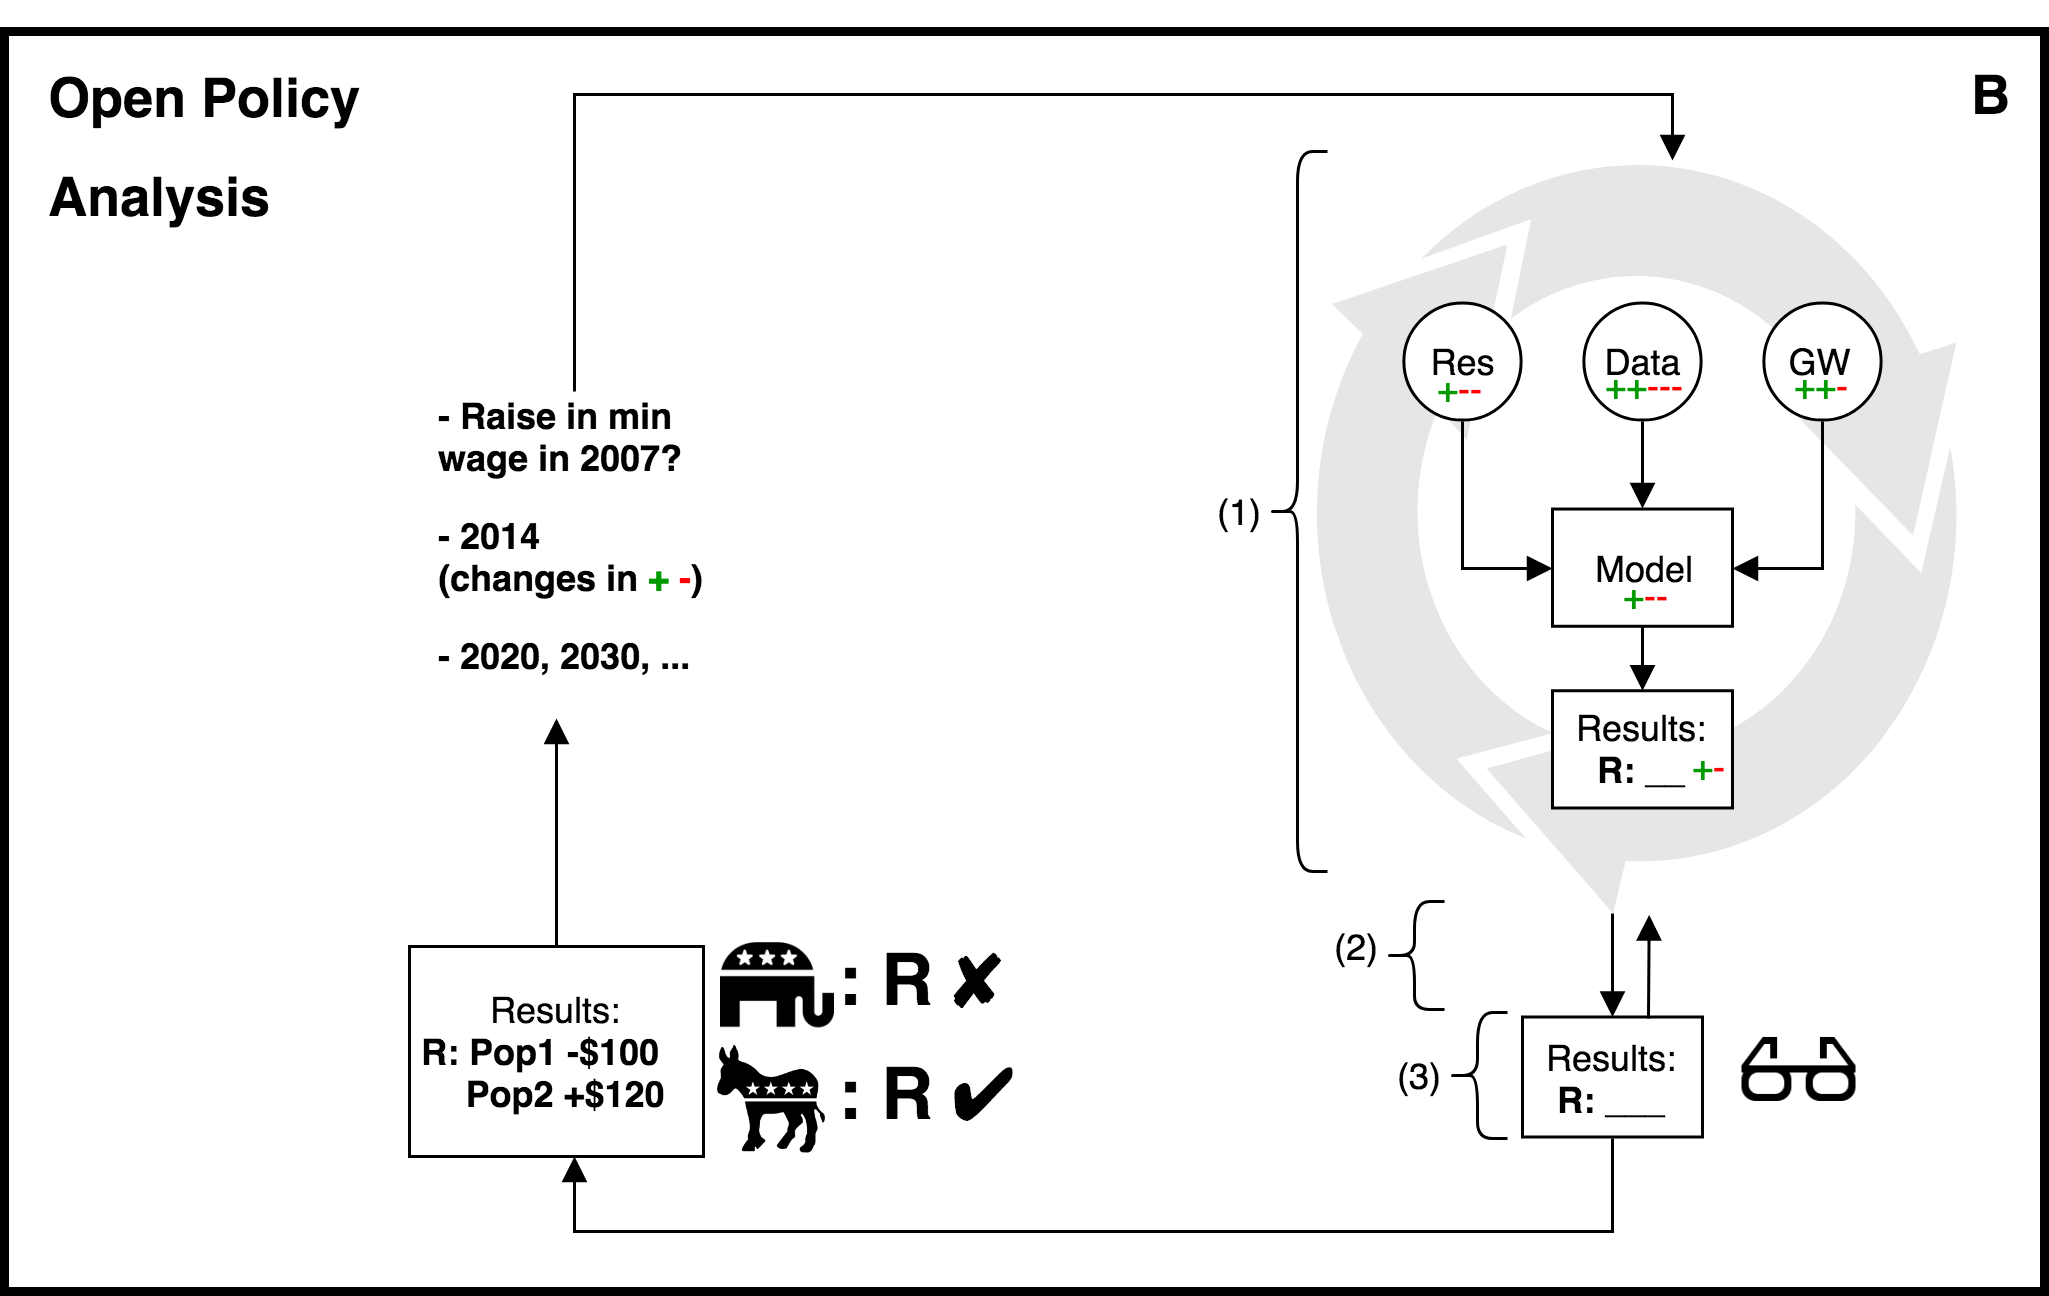
\includegraphics[width=.86\paperwidth]{../Images/open_pa.PNG}
       };
   \end{tikzpicture}
\end{frame}

\begin{frame}{Conclusion}
\begin{itemize}
\item Draw a parallel between reproducibility crisis in empirical research and a credibility crisis in policy analysis. 
\item Proposed guiding principles for open policy analysis.
\item Identify challenges and provide recommendations for different stakeholders.
\end{itemize}
\end{frame}


\begin{frame}{Next Steps} 
\begin{itemize}
\item Journal Science was key for research. Need high profile producer of policy analysis to buy in. 
\item Develop community endorsed guidelines for OPA (similar to TOP Guidelines for Open Science)
\item Carry out case studies with policy agencies to fine tune guidelines, and build a collection of examples (Hoces de la Guardia 2017). 
\end{itemize}
\end{frame} 

\begin{frame}[noframenumbering]
\begin{center}
\vspace*{4em}
{\Large Thank you.\\}
\bigskip
Pre-print: [PP URL HERE]   \\
Contact:  \href{mailto:fhoces@berkeley.edu}{fhoces@berkeley.edu}

\end{center}
\end{frame}

\end{document}

